\documentclass{article}
\usepackage[letterpaper]{geometry}
\usepackage{fullpage}
\usepackage{amsmath}
\usepackage{amssymb}
\usepackage{graphicx}
\usepackage{wrapfig}
\usepackage{float}
\usepackage{color}
\usepackage{booktabs}
\usepackage{epstopdf}
\usepackage{subcaption}

\usepackage{fixltx2e}

\usepackage{hyperref}
\hypersetup{
    pdftitle={Sig-Fi Overview},
    pdfauthor={Joel D. Brinton},
    pdfsubject={Sig-Fi Overview},
    pdfkeywords={SigLabs, Signal Laboratories, Inc., Sig-Fi, SigFi},
    bookmarksnumbered=true,
    bookmarksopen=true,
    bookmarksopenlevel=3,
    colorlinks=true,
    pdfpagemode=UseOutlines
}
\usepackage{hypcap}

\usepackage{helvet}
\renewcommand*\familydefault{\sfdefault} %% Only if the base font of the document is to be sans serif
\usepackage[T1]{fontenc}

%\setlength({\droptitle}{-10em}
\graphicspath{{../assets/}}


\title{\begin{center}

\includegraphics[scale=0.5]{logo2-normal-draft.eps}
\end{center}
Copper Suicide\textsuperscript{\texttrademark} User Manual\\
Scalable FPGA Development Board\\
% \subtitle{High Dynamic Range Radio with\\Split Ring Resonator-loaded MIMO Antenna}
\author{Joel D. Brinton\\Signal Laboratories, Inc.}}
% \date{July 1, 2014}

\newcommand{\designator}[1]{\textbf{\texttt{#1}}}

\begin{document}


\maketitle
\section{Abstract}

Copper Suicide is a scalable FPGA development board based on the Lattice Semiconductor ECP5 FPGA. It consists of an Arm Cortex-M7 processor, 1 configuration FPGA, 8 gigabytes of DDR3 SDRAM, and 16 general purpose FPGAs in a square 2-dimensional architecture. The design measures 200x200 mm and is extensible by stacking additional boards on top or bottom.

\newpage

\section{Overview}

Copper Suicide is designed to have the most flexibility between interconnections, and the highest data rate. There are 3 primary ways to communicate with the FPGA. First, each chip has 4 edge buses. These connect to adjacent FPGA's. On the left/right board edges they connect to DRAM chips. On the top/bottom board edges they connect to  either top or bottom board-to-board connectors. Second, the Memory and Interupt Bus (MIB) is a 29-pin multi-drop bus which connects all 17 FPGAs. Third, there is a 5-pin programming bus connecting each FPGA to the configuration FPGA.

There is an additional 41-bit SRAM memory interface between the MCU and configuration FPGA. This bus may also be used as a general purpose interface between the MCU and configuration FPGA.

There are two more dedicated MIB from the configuration FPGA, one to the bottom board connector and one to the top.

Also, each FPGA has a dedicated point-of-presence power supply controller which allows monitoring and adjustment of individual FPGA current and voltages. Global power supply voltages and currents are also monitored.

Finally, 128 megabytes of NOR Flash is provided on the configuration FPGA, and 256 megabytes on the MCU. Indicator LEDs are connected to the MCU and each FPGA.


\subsection{Block Diagram}

The FPGA block diagram, Figure \ref{fig:blockdiagram}, shows all FPGA and ARM connections.

\begin{figure}[H]
  \centering
  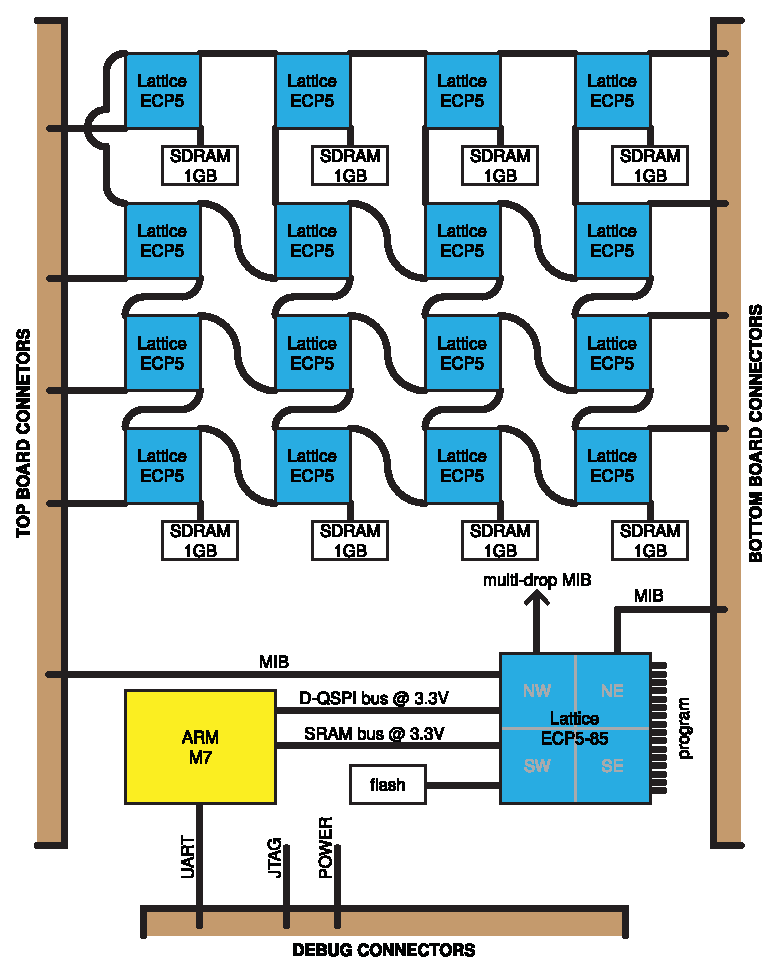
\includegraphics[scale=1]{cs_block_diagram.eps}
  \caption{Copper Suicide Block Diagram}
  \label{fig:blockdiagram}
\end{figure}

\subsection{FPGA Harnesses}

For simplicity of design, all FPGAs share the same schematic. Figure \ref{fig:fpga} shows the FPGA interconnections. Figure \ref{fig:harness} shows the harness wiring bundles.

\begin{figure}[H]
  \centering
  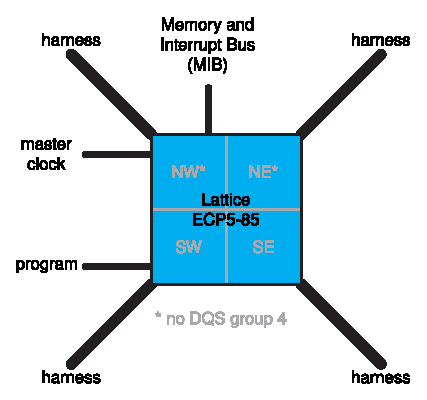
\includegraphics[scale=1]{cs_fpga.eps}
	\caption{Copper Suicide FPGA}
	\label{fig:fpga}
\end{figure}

\begin{figure}[H]
  \centering
  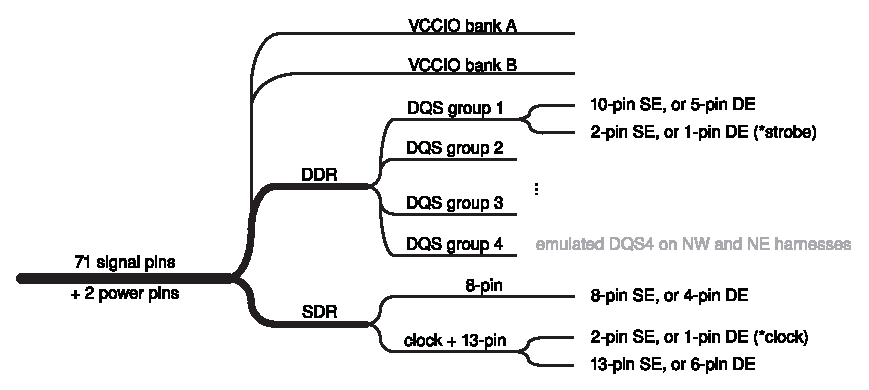
\includegraphics[scale=1]{cs_harness.eps}
	\caption{Copper Suicide Harness}
	\label{fig:harness}
\end{figure}




\newpage

\subsection{JTAG}

The JTAG daisy-chain starts with the MCU and then connects to the configuration FPGA and then the rest of the array, figure \ref{fig:jtagdaisy}. Each device may be removed from the daisy chain with jumpers on the side of the board. If there is a need to connect to a single device the same jumpers may be used as a direct JTAG connection. The daisy-chain loops back around from the last FPGA in the array to the MCU.

By default the MCU disables JTAG and instead uses SWD programming. When in SWD mode the MCU must be bypassed to read from the array.

\begin{figure}[H]
  \centering
  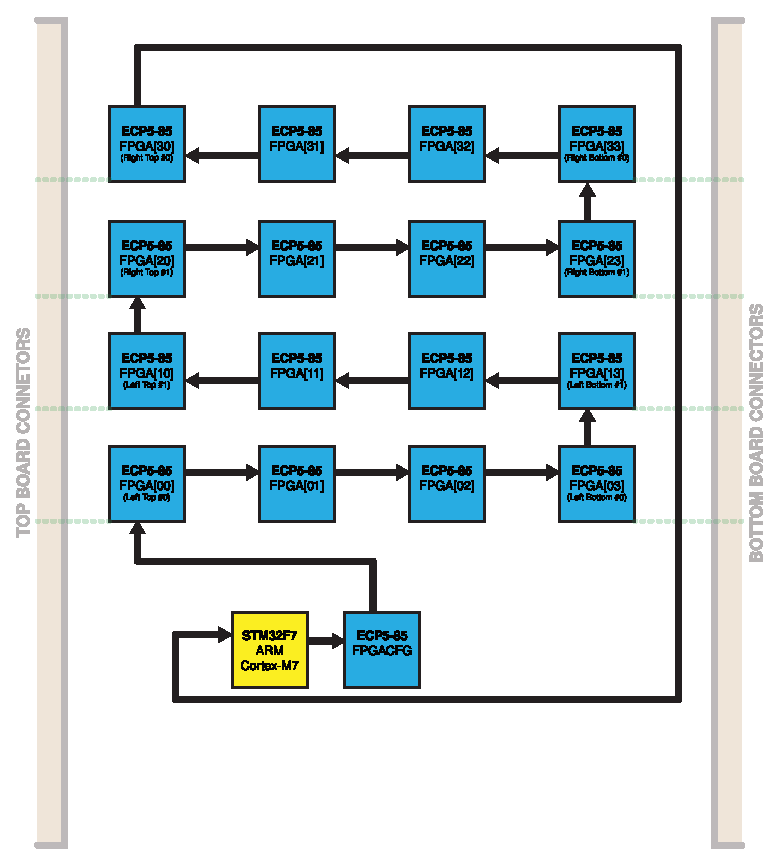
\includegraphics[scale=1]{jtag_daisy.eps}
  \caption{Copper Suicide JTAG Block Diagram}
  \label{fig:jtagdaisy}
\end{figure}

\subsubsection{headers}

There are 18 JTAG connectors which include the MCU, the configuration FPGA, and the 16 FPGA arrray. The connectors are 10-pin, 50mil pitch, male, unshrouded right-angle thru-hole connectors (Sullins part number GRPB052VWVN).

\begin{figure}[H]
  \centering
  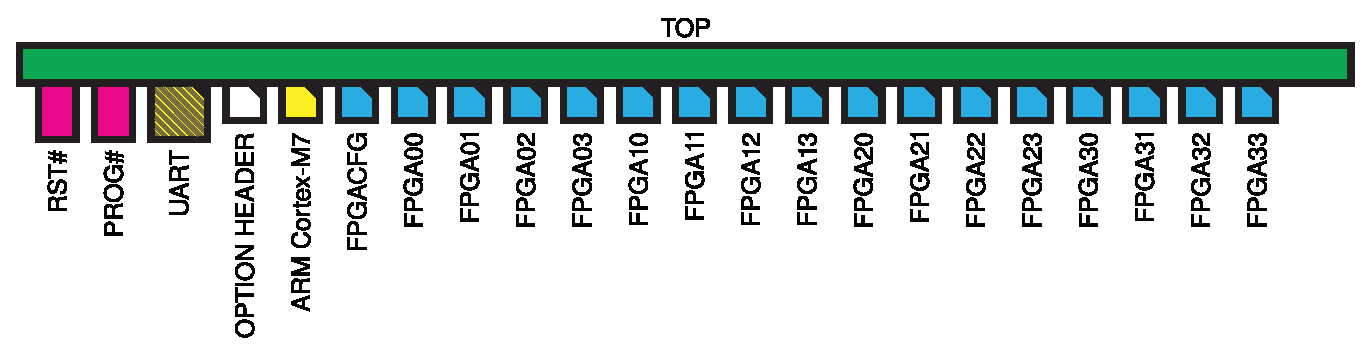
\includegraphics[scale=0.6]{cs_headers.eps}
  \caption{Copper Suicide Debug Headers}
  \label{fig:debugheaders}
\end{figure}

They can be jumpered (inserted into the daisy chain) or bypassed (taken out of the daisy chain) with 50mil pitch jumpers (Harwin P/N M50-2000005).


\begin{figure}[H]
  \centering
  \begin{subfigure}{0.5\textwidth}
    \centering
    \includegraphics[width=0.8\linewidth]{cs_jtag_daisy}
    \caption{JTAG daisy-chain jumper configuration}
    \label{fig:csjtagdaisy}
  \end{subfigure}%
  \begin{subfigure}{0.5\textwidth}
    \centering
    \includegraphics[width=0.8\linewidth]{cs_jtag_bypass}
    \caption{JTAG bypass jumper configuration}
    \label{fig:csjtagbypass}
  \end{subfigure}
\end{figure}


\subsubsection{JTAG Adapter Cables}


The JTAG connectors are non standard and an adapter cable is used to connect it to the Lattice provided JTAG programmer (Lattice P/N HW-USBN-2B). There are two JTAG Adapter Cables. First, a non-daisy chain cable shorts the daisy-chain loop and allows the programmer to access just one device. Second, a daisy-chain programming cable connects to all devices which have been connected in the chain. The JTAG adapter cables use 50mil pitch female connectors (Amphenol/FCI part number 20021311-00010T4LF).

\begin{figure}[H]
  \centering
  \begin{subfigure}{0.5\textwidth}
    \centering
    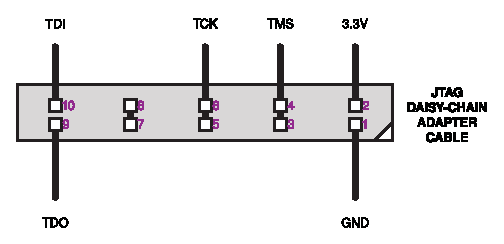
\includegraphics[width=0.8\linewidth]{cs_jtag_daisy-chain_adapter_cable}
    \caption{JTAG daisy-chain cable}
    \label{fig:jtagdaisychaincable}
  \end{subfigure}%
  \begin{subfigure}{0.5\textwidth}
    \centering
    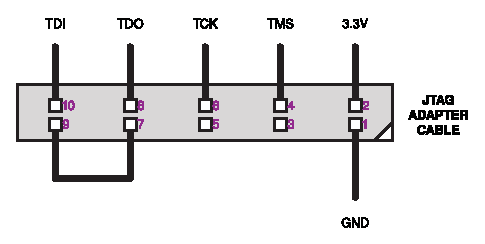
\includegraphics[width=0.8\linewidth]{cs_jtag_adapter_cable}
    \caption{JTAG cable}
    \label{fig:jtagcable}
  \end{subfigure}
\end{figure}



%%\section{Pinouts}
%%
%%\section{Troubleshooting}
%%
%%JTAG is giving readback errors : check that the TMS net is pulled up and TCK net is pulled down. Even if you are using the JTAG adapter in "direct connect" mode (as opposed to "daisy chain" mode) the board needs to be in loopback mode (J6 needs to be jumpered, pin 1 to pin 2, and pin 3 to pin 4).
%%
%%MCU is not programming :  make sure to unlock the MCU using the instructions in \S\ref{mcuunlock}.



\end{document}
